% =====================================================================
% Figure 4 -- Miss-rate / intervention-rate Pareto trade-off
%   fixes: (1) cost row no longer spills outside the axes
%          (2) no text over the curve; callout box is translucent
%          (3) zero-miss frontier labelled once, clear of the tau tags
% RESS compliant: vector, colourblind-safe, >=8 pt lettering
% Compile: pdflatex fig4_pareto.tex
% =====================================================================
\documentclass[border=6pt]{standalone}
\usepackage[T1]{fontenc}
\usepackage[scaled=0.95]{helvet}
\renewcommand{\familydefault}{\sfdefault}
\usepackage{amsmath}
\usepackage{pgfplots}
\pgfplotsset{compat=1.18}
\usetikzlibrary{calc}
\newcommand{\tC}{\fontsize{8.4}{10.2}\selectfont}
\newcommand{\tD}{\fontsize{9.6}{11.4}\selectfont}
\begin{document}
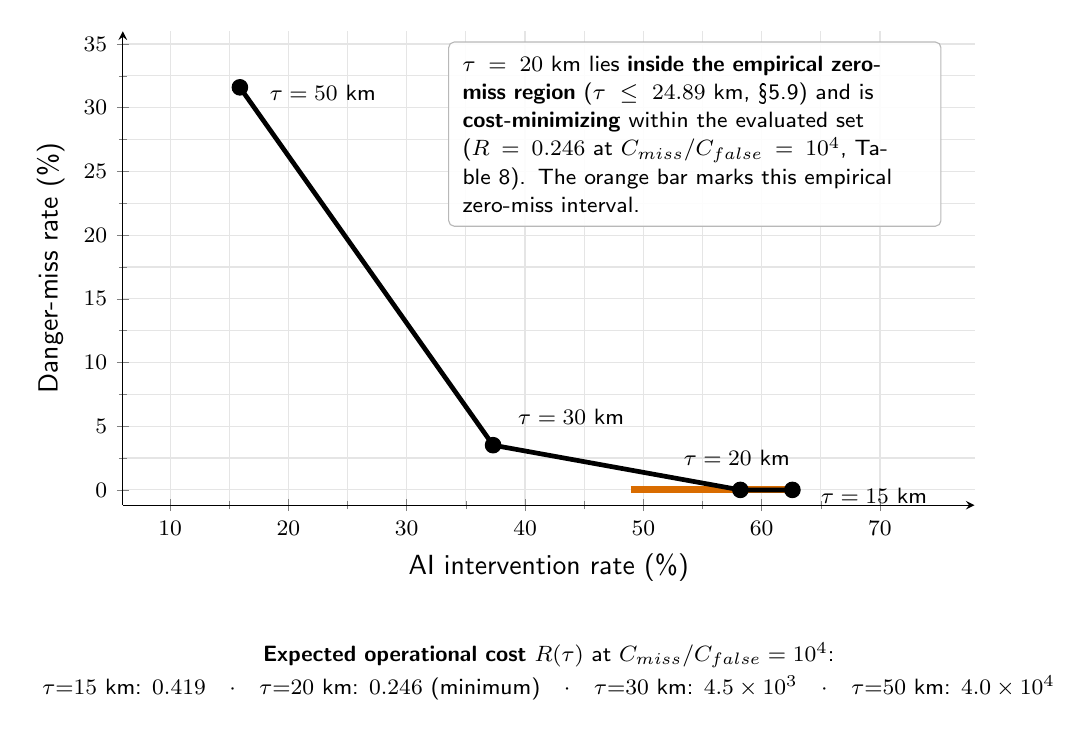
\begin{tikzpicture}
\begin{axis}[
  name=ax,
  width=12.4cm, height=7.6cm,
  xlabel={AI intervention rate (\%)},
  ylabel={Danger-miss rate (\%)},
  xmin=6, xmax=78, ymin=-1.2, ymax=36,
  xtick={10,20,30,40,50,60,70}, ytick={0,5,10,15,20,25,30,35},
  minor tick num=1,
  grid=both, grid style={draw=black!10},
  tick label style={font=\tC}, label style={font=\tD},
  axis lines=left,
]
% ---------- empirical zero-miss interval : slim bar sitting ON the axis ----------
\draw[orange!85!black,line width=2.6pt,line cap=butt]
      (axis cs:48.93,0.06) -- (axis cs:62.61,0.06);
% ---------- Pareto curve (drawn AFTER the band -> on top) ----------
\addplot[black,line width=1.7pt,forget plot]
  coordinates {(15.9,31.6) (37.3,3.51) (58.2,0) (62.6,0)};
\addplot[only marks,mark=*,mark size=2.8pt,black,forget plot]
  coordinates {(15.9,31.6) (37.3,3.51) (58.2,0) (62.6,0)};
% ---------- threshold tags (all clear of the curve) ----------
\node[font=\tC,anchor=west]  at (axis cs:17.6,31.2) {$\tau=50$ km};
\node[font=\tC,anchor=south west] at (axis cs:38.6,4.4) {$\tau=30$ km};
\node[font=\tC,anchor=south] at (axis cs:57.9,1.15) {$\tau=20$ km};
\node[font=\tC,anchor=west]  at (axis cs:64.2,-0.45) {$\tau=15$ km};
% ---------- callout : upper-right corner, empty region, translucent ----------
\node[draw=black!28,fill=white,fill opacity=0.92,text opacity=1,
      rounded corners=2pt,inner sep=5pt,font=\tC,align=left,
      text width=5.9cm,anchor=north west] at (axis cs:33.5,35.2)
  {$\tau=20$ km lies \textbf{inside the empirical zero-miss region}
   ($\tau\le24.89$ km, \S5.9) and is \textbf{cost-minimizing} within the
   evaluated set ($R=0.246$ at $C_{miss}/C_{false}=10^{4}$, Table~8).
   The orange bar marks this empirical zero-miss interval.};
\end{axis}
% ---------- cost row : OUTSIDE the axes, under the x-label ----------
\node[font=\tC,align=center,anchor=north] at ([yshift=-1.62cm]ax.south)
  {\textbf{Expected operational cost} $R(\tau)$ at $C_{miss}/C_{false}=10^{4}$:\\[2pt]
   $\tau{=}15$ km: $0.419$\quad$\cdot$\quad
   $\tau{=}20$ km: $0.246$ (minimum)\quad$\cdot$\quad
   $\tau{=}30$ km: $4.5\times10^{3}$\quad$\cdot$\quad
   $\tau{=}50$ km: $4.0\times10^{4}$};
\end{tikzpicture}
\end{document}
